\documentclass[twoside]{book}

% Packages required by doxygen
\usepackage{fixltx2e}
\usepackage{calc}
\usepackage{doxygen}
\usepackage[export]{adjustbox} % also loads graphicx
\usepackage{graphicx}
\usepackage[utf8]{inputenc}
\usepackage{makeidx}
\usepackage{multicol}
\usepackage{multirow}
\PassOptionsToPackage{warn}{textcomp}
\usepackage{textcomp}
\usepackage[nointegrals]{wasysym}
\usepackage[table]{xcolor}

% Font selection
\usepackage[T1]{fontenc}
\usepackage[scaled=.90]{helvet}
\usepackage{courier}
\usepackage{amssymb}
\usepackage{sectsty}
\renewcommand{\familydefault}{\sfdefault}
\allsectionsfont{%
  \fontseries{bc}\selectfont%
  \color{darkgray}%
}
\renewcommand{\DoxyLabelFont}{%
  \fontseries{bc}\selectfont%
  \color{darkgray}%
}
\newcommand{\+}{\discretionary{\mbox{\scriptsize$\hookleftarrow$}}{}{}}

% Page & text layout
\usepackage{geometry}
\geometry{%
  a4paper,%
  top=2.5cm,%
  bottom=2.5cm,%
  left=2.5cm,%
  right=2.5cm%
}
\tolerance=750
\hfuzz=15pt
\hbadness=750
\setlength{\emergencystretch}{15pt}
\setlength{\parindent}{0cm}
\setlength{\parskip}{3ex plus 2ex minus 2ex}
\makeatletter
\renewcommand{\paragraph}{%
  \@startsection{paragraph}{4}{0ex}{-1.0ex}{1.0ex}{%
    \normalfont\normalsize\bfseries\SS@parafont%
  }%
}
\renewcommand{\subparagraph}{%
  \@startsection{subparagraph}{5}{0ex}{-1.0ex}{1.0ex}{%
    \normalfont\normalsize\bfseries\SS@subparafont%
  }%
}
\makeatother

% Headers & footers
\usepackage{fancyhdr}
\pagestyle{fancyplain}
\fancyhead[LE]{\fancyplain{}{\bfseries\thepage}}
\fancyhead[CE]{\fancyplain{}{}}
\fancyhead[RE]{\fancyplain{}{\bfseries\leftmark}}
\fancyhead[LO]{\fancyplain{}{\bfseries\rightmark}}
\fancyhead[CO]{\fancyplain{}{}}
\fancyhead[RO]{\fancyplain{}{\bfseries\thepage}}
\fancyfoot[LE]{\fancyplain{}{}}
\fancyfoot[CE]{\fancyplain{}{}}
\fancyfoot[RE]{\fancyplain{}{\bfseries\scriptsize Generated by Doxygen }}
\fancyfoot[LO]{\fancyplain{}{\bfseries\scriptsize Generated by Doxygen }}
\fancyfoot[CO]{\fancyplain{}{}}
\fancyfoot[RO]{\fancyplain{}{}}
\renewcommand{\footrulewidth}{0.4pt}
\renewcommand{\chaptermark}[1]{%
  \markboth{#1}{}%
}
\renewcommand{\sectionmark}[1]{%
  \markright{\thesection\ #1}%
}

% Indices & bibliography
\usepackage{natbib}
\usepackage[titles]{tocloft}
\setcounter{tocdepth}{3}
\setcounter{secnumdepth}{5}
\makeindex

% Hyperlinks (required, but should be loaded last)
\usepackage{ifpdf}
\ifpdf
  \usepackage[pdftex,pagebackref=true]{hyperref}
\else
  \usepackage[ps2pdf,pagebackref=true]{hyperref}
\fi
\hypersetup{%
  colorlinks=true,%
  linkcolor=blue,%
  citecolor=blue,%
  unicode%
}

% Custom commands
\newcommand{\clearemptydoublepage}{%
  \newpage{\pagestyle{empty}\cleardoublepage}%
}

\usepackage{caption}
\captionsetup{labelsep=space,justification=centering,font={bf},singlelinecheck=off,skip=4pt,position=top}

%===== C O N T E N T S =====

\begin{document}

% Titlepage & ToC
\hypersetup{pageanchor=false,
             bookmarksnumbered=true,
             pdfencoding=unicode
            }
\pagenumbering{roman}
\begin{titlepage}
\vspace*{7cm}
\begin{center}%
{\Large My Project }\\
\vspace*{1cm}
{\large Generated by Doxygen 1.8.11}\\
\end{center}
\end{titlepage}
\clearemptydoublepage
\tableofcontents
\clearemptydoublepage
\pagenumbering{arabic}
\hypersetup{pageanchor=true}

%--- Begin generated contents ---
\chapter{File Index}
\section{File List}
Here is a list of all documented files with brief descriptions\+:\begin{DoxyCompactList}
\item\contentsline{section}{\hyperlink{enigm_8c}{enigm.\+c} }{\pageref{enigm_8c}}{}
\item\contentsline{section}{{\bfseries enigm.\+h} }{\pageref{enigm_8h}}{}
\item\contentsline{section}{\hyperlink{main_8c}{main.\+c} }{\pageref{main_8c}}{}
\end{DoxyCompactList}

\chapter{File Documentation}
\hypertarget{enigm_8c}{}\section{enigm.\+c File Reference}
\label{enigm_8c}\index{enigm.\+c@{enigm.\+c}}
{\ttfamily \#include $<$stdio.\+h$>$}\\*
{\ttfamily \#include $<$stdlib.\+h$>$}\\*
{\ttfamily \#include $<$string.\+h$>$}\\*
{\ttfamily \#include \char`\"{}time.\+h\char`\"{}}\\*
{\ttfamily \#include \char`\"{}S\+D\+L/\+S\+D\+L.\+h\char`\"{}}\\*
{\ttfamily \#include $<$math.\+h$>$}\\*
{\ttfamily \#include \char`\"{}S\+D\+L/\+S\+D\+L\+\_\+ttf.\+h\char`\"{}}\\*
{\ttfamily \#include \char`\"{}enigm.\+h\char`\"{}}\\*
Include dependency graph for enigm.\+c\+:
\nopagebreak
\begin{figure}[H]
\begin{center}
\leavevmode
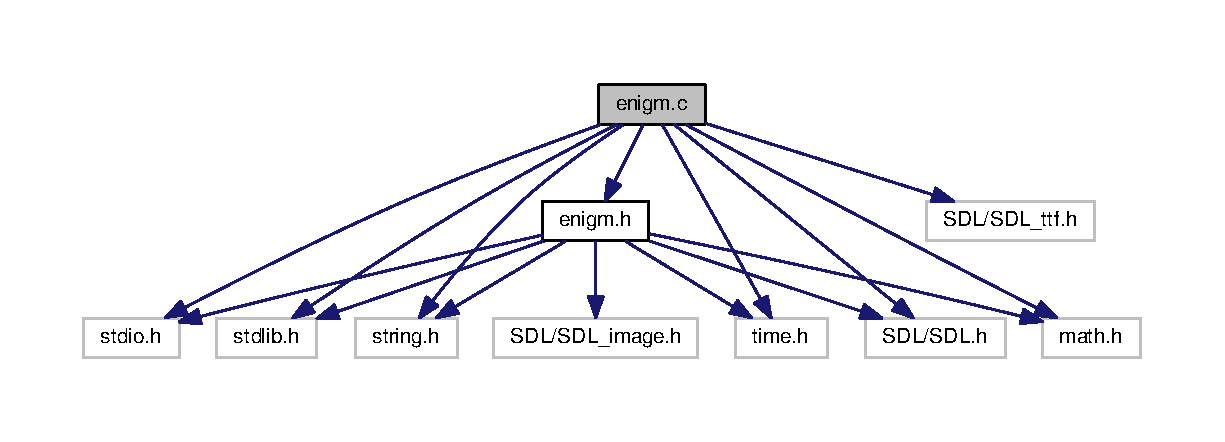
\includegraphics[width=350pt]{enigm_8c__incl}
\end{center}
\end{figure}
\subsection*{Functions}
\begin{DoxyCompactItemize}
\item 
int \hyperlink{enigm_8c_ab39701330d5b5e53de75d2dc02a32e09}{generate\+\_\+question} (int $\ast$n)
\begin{DoxyCompactList}\small\item\em to generate random number \end{DoxyCompactList}\item 
void \hyperlink{enigm_8c_a39136b881876a011385cbcbdb602cbba}{init\+\_\+affichier\+\_\+question} (int n, S\+D\+L\+\_\+\+Surface $\ast$screen)
\begin{DoxyCompactList}\small\item\em to show the question \end{DoxyCompactList}\item 
int {\bfseries resolution} (int n)\hypertarget{enigm_8c_aec0359022ae32346ca1b43fc38e922d6}{}\label{enigm_8c_aec0359022ae32346ca1b43fc38e922d6}

\item 
int \hyperlink{enigm_8c_a44acf4738d676b7f25d62cefca694cc1}{reponse} (int $\ast$rep)
\begin{DoxyCompactList}\small\item\em to give the right answer \end{DoxyCompactList}\item 
void {\bfseries afficher\+\_\+resultat} (S\+D\+L\+\_\+\+Surface $\ast$screen, int solution, int r)\hypertarget{enigm_8c_ab6b2c779523bee2c73a0f16ba9f49253}{}\label{enigm_8c_ab6b2c779523bee2c73a0f16ba9f49253}

\end{DoxyCompactItemize}


\subsection{Function Documentation}
\index{enigm.\+c@{enigm.\+c}!generate\+\_\+question@{generate\+\_\+question}}
\index{generate\+\_\+question@{generate\+\_\+question}!enigm.\+c@{enigm.\+c}}
\subsubsection[{\texorpdfstring{generate\+\_\+question(int $\ast$n)}{generate_question(int *n)}}]{\setlength{\rightskip}{0pt plus 5cm}int generate\+\_\+question (
\begin{DoxyParamCaption}
\item[{int $\ast$}]{n}
\end{DoxyParamCaption}
)}\hypertarget{enigm_8c_ab39701330d5b5e53de75d2dc02a32e09}{}\label{enigm_8c_ab39701330d5b5e53de75d2dc02a32e09}


to generate random number 


\begin{DoxyParams}{Parameters}
{\em n} & the number \\
\hline
\end{DoxyParams}
\begin{DoxyReturn}{Returns}
a the number 
\end{DoxyReturn}
\index{enigm.\+c@{enigm.\+c}!init\+\_\+affichier\+\_\+question@{init\+\_\+affichier\+\_\+question}}
\index{init\+\_\+affichier\+\_\+question@{init\+\_\+affichier\+\_\+question}!enigm.\+c@{enigm.\+c}}
\subsubsection[{\texorpdfstring{init\+\_\+affichier\+\_\+question(int n, S\+D\+L\+\_\+\+Surface $\ast$screen)}{init_affichier_question(int n, SDL_Surface *screen)}}]{\setlength{\rightskip}{0pt plus 5cm}void init\+\_\+affichier\+\_\+question (
\begin{DoxyParamCaption}
\item[{int}]{n, }
\item[{S\+D\+L\+\_\+\+Surface $\ast$}]{screen}
\end{DoxyParamCaption}
)}\hypertarget{enigm_8c_a39136b881876a011385cbcbdb602cbba}{}\label{enigm_8c_a39136b881876a011385cbcbdb602cbba}


to show the question 


\begin{DoxyParams}{Parameters}
{\em n} & the number , screen \\
\hline
\end{DoxyParams}
\begin{DoxyReturn}{Returns}
nothing 
\end{DoxyReturn}
\index{enigm.\+c@{enigm.\+c}!reponse@{reponse}}
\index{reponse@{reponse}!enigm.\+c@{enigm.\+c}}
\subsubsection[{\texorpdfstring{reponse(int $\ast$rep)}{reponse(int *rep)}}]{\setlength{\rightskip}{0pt plus 5cm}int reponse (
\begin{DoxyParamCaption}
\item[{int $\ast$}]{rep}
\end{DoxyParamCaption}
)}\hypertarget{enigm_8c_a44acf4738d676b7f25d62cefca694cc1}{}\label{enigm_8c_a44acf4738d676b7f25d62cefca694cc1}


to give the right answer 


\begin{DoxyParams}{Parameters}
{\em rep} & the number \\
\hline
\end{DoxyParams}
\begin{DoxyReturn}{Returns}
b the number 
\end{DoxyReturn}

\hypertarget{main_8c}{}\section{main.\+c File Reference}
\label{main_8c}\index{main.\+c@{main.\+c}}
{\ttfamily \#include $<$stdio.\+h$>$}\\*
{\ttfamily \#include $<$stdlib.\+h$>$}\\*
{\ttfamily \#include $<$string.\+h$>$}\\*
{\ttfamily \#include \char`\"{}time.\+h\char`\"{}}\\*
{\ttfamily \#include \char`\"{}S\+D\+L/\+S\+D\+L.\+h\char`\"{}}\\*
{\ttfamily \#include $<$math.\+h$>$}\\*
{\ttfamily \#include \char`\"{}enigm.\+h\char`\"{}}\\*
{\ttfamily \#include \char`\"{}S\+D\+L/\+S\+D\+L\+\_\+ttf.\+h\char`\"{}}\\*
Include dependency graph for main.\+c\+:\nopagebreak
\begin{figure}[H]
\begin{center}
\leavevmode
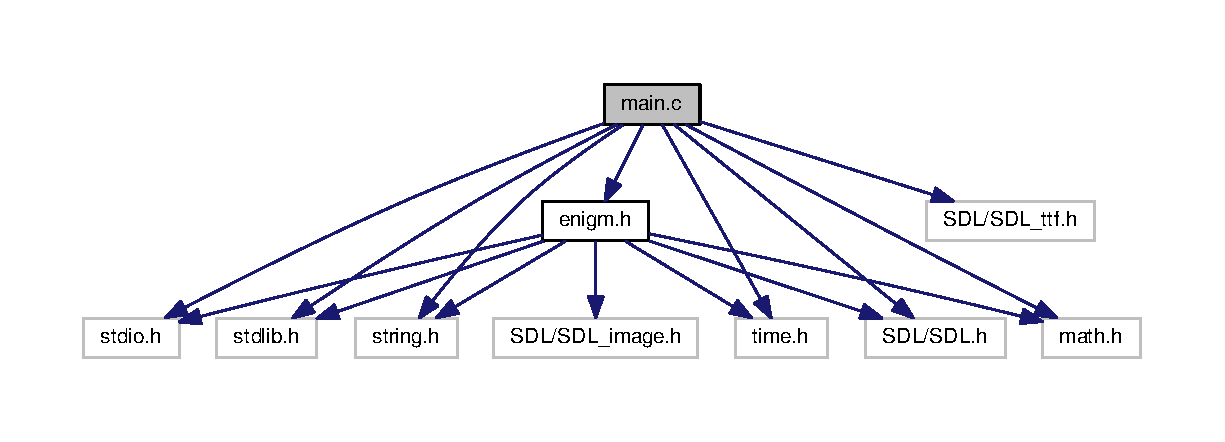
\includegraphics[width=350pt]{main_8c__incl}
\end{center}
\end{figure}
\subsection*{Functions}
\begin{DoxyCompactItemize}
\item 
int {\bfseries main} (void)\hypertarget{main_8c_a840291bc02cba5474a4cb46a9b9566fe}{}\label{main_8c_a840291bc02cba5474a4cb46a9b9566fe}

\end{DoxyCompactItemize}

%--- End generated contents ---

% Index
\backmatter
\newpage
\phantomsection
\clearemptydoublepage
\addcontentsline{toc}{chapter}{Index}
\printindex

\end{document}
